\documentclass[11pt,a4paper]{article}

% =========================================================
% PACKAGES
% =========================================================
\usepackage[utf8]{inputenc}
\usepackage[T1]{fontenc}
\usepackage{lmodern}
\usepackage[a4paper,margin=2.2cm]{geometry}

\usepackage{amsmath,amssymb}
\usepackage{booktabs}
\usepackage{array}
\usepackage{longtable}
\usepackage{multirow}
\usepackage{graphicx}
\usepackage{float}
\usepackage{caption}
\usepackage{subcaption}
\usepackage{xcolor}
\usepackage{enumitem}
\usepackage{microtype}
\usepackage{setspace}
\usepackage{titlesec}
\usepackage{fancyhdr}

\usepackage[hidelinks]{hyperref}
\usepackage{bookmark}

\usepackage{tikz}
\usepackage{pgfplots}
\usepackage{adjustbox}
\usepackage{tabularx}

\usetikzlibrary{shapes.geometric, arrows.meta, positioning}

\pgfplotsset{compat=1.18}

% =========================================================
% DOCUMENT SETTINGS
% =========================================================
\onehalfspacing
\setlength{\parindent}{0pt}
\setlength{\parskip}{5pt}

\hypersetup{
    colorlinks=true,
    linkcolor=black,
    citecolor=black,
    urlcolor=blue,
    pdftitle={Data-Driven Customer Analytics for E-Commerce Decision Making},
    pdfauthor={Mahdiyeh Mirzaei}
}

% =========================================================
% HEADER / FOOTER
% =========================================================
\pagestyle{fancy}
\fancyhf{}
\lhead{\small Customer Analytics for E-Commerce}
\rhead{\small Mahdiyeh Mirzaei}
\cfoot{\thepage}
\renewcommand{\headrulewidth}{0.4pt}

% =========================================================
% SECTION STYLE
% =========================================================
\titleformat{\section}
{\large\bfseries}
{\thesection.}
{0.6em}
{}

\titleformat{\subsection}
{\normalsize\bfseries}
{\thesubsection.}
{0.6em}
{}

\titleformat{\subsubsection}
{\normalsize\itshape}
{\thesubsubsection.}
{0.6em}
{}

\titlespacing*{\section}{0pt}{18pt}{8pt}
\titlespacing*{\subsection}{0pt}{12pt}{5pt}

% =========================================================
% TABLE SETTINGS
% =========================================================
\captionsetup{
    font=small,
    labelfont=bf,
    justification=centering
}

\renewcommand{\arraystretch}{1.2}

% =========================================================
% CUSTOM COMMANDS
% =========================================================
\newcommand{\Hnull}{H_{0}}
\newcommand{\Halt}{H_{1}}

% =========================================================
% DOCUMENT
% =========================================================
\begin{document}

% =========================================================
% TITLE PAGE
% =========================================================

\begin{titlepage}
\centering

\vspace*{1.5cm}

{\Large\bfseries Data-Driven Customer Analytics for E-Commerce Decision Making\par}

\vspace{0.7cm}

{\large\itshape An Integrated Statistical and Machine-Learning Approach to Customer Value, Churn Risk, Segmentation, and Marketing Optimization\par}

\vspace{1.8cm}

\begin{tikzpicture}
\node[
    draw,
    rounded rectangle,
    minimum width=10cm,
    minimum height=1.2cm,
    align=center
]
{
\textbf{Project 2}\\
Customer Analytics for E-Commerce
};
\end{tikzpicture}

\vfill

{\large
\textbf{Author}\\[0.2cm]
Mahdiyeh Mirzaei
\par}

\vspace{0.5cm}

{\large
\textbf{Team / Community}\\[0.2cm]
StudyBuild Community
\par}

\vspace{0.5cm}

\href{https://github.com/mahdiyeh-mirzaei-v2}
{github.com/mahdiyeh-mirzaei-v2}

\vspace{0.15cm}

\href{https://github.com/StudyBuildCommunity}
{github.com/StudyBuildCommunity}

\vfill

{\large
\textbf{2026}
\par}

\end{titlepage}

% =========================================================
% ABSTRACT
% =========================================================

\section*{Abstract}
\addcontentsline{toc}{section}{Abstract}

This study presents an integrated customer analytics framework for an e-commerce company using statistical analysis, unsupervised learning, and supervised machine learning. The analytical dataset contains 60 customers and 26 original variables covering demographic, transactional, behavioral, and satisfaction-related characteristics. The methodology combines exploratory data analysis, descriptive statistics, normality testing, Interquartile Range (IQR)-based outlier detection, Spearman rank correlation, customer value scoring, K-Means clustering, non-parametric hypothesis testing, churn-risk classification, and predictive modeling.

The results indicate substantial heterogeneity in customer economic value. Customers were divided into three equally sized value groups, including 20 High-Value, 20 Medium-Value, and 20 Low-Value customers. A total of 36 customers, corresponding to 60\% of the sample, were classified as churn-risk customers using an inactivity threshold of more than 180 days. Importantly, 12 customers were simultaneously classified as High Value and Churn Risk, identifying a strategically critical retention group.

K-Means clustering identified three behavioral segments. The most valuable cluster consisted of only six customers but exhibited an average total spending of approximately 14,188.76. The Kruskal--Wallis test confirmed statistically significant differences in spending distributions across clusters ($H=16.109$, $p=0.000318$).

The discount analysis did not identify a statistically significant difference in spending between customers using discounts and those not using discounts. The Mann--Whitney U test resulted in $U=391$ and $p=0.4512$. The machine-learning analysis also produced limited predictive performance, with mean cross-validated ROC-AUC values of approximately 0.564 for Logistic Regression and 0.478 for Random Forest.

At the geographical level, Mashhad generated the highest observed total revenue of approximately 64,118.44 and obtained the highest marketing opportunity score. Based on these findings, the study recommends prioritizing high-value churn-risk customers, increasing average order value among frequent low-basket customers, and validating marketing investment in Mashhad through controlled experimentation.

\textbf{Keywords:} Customer Analytics; E-Commerce; Customer Value; Churn Risk; K-Means; Logistic Regression; Random Forest; Spearman Correlation; Non-Parametric Statistics; Marketing Analytics.

% =========================================================
% TABLE OF CONTENTS
% =========================================================

\newpage
\tableofcontents
\newpage

% =========================================================
% 1 INTRODUCTION
% =========================================================

\section{Introduction}

The rapid expansion of e-commerce has created large volumes of customer-level data containing information about purchasing behavior, transaction value, customer satisfaction, discounts, returns, and demographic characteristics. The availability of such data provides organizations with an opportunity to move from intuition-based marketing toward evidence-based decision making.

However, raw customer data do not directly provide managerial insight. Organizations must identify economically valuable customers, recognize inactive or potentially lost customers, understand heterogeneous behavioral patterns, and determine where marketing resources are most likely to generate incremental value.

The central research question of this project is:

\begin{quote}
\textit{How can customer-level behavioral and transactional data be transformed into statistically supported and actionable strategies for improving customer retention, revenue generation, and marketing efficiency?}
\end{quote}

The analysis addresses five principal managerial questions:

\begin{enumerate}[label=\arabic*.]
    \item Which customers generate the greatest economic value?
    \item Which customers are potentially at risk of becoming inactive?
    \item Which customer segments exhibit distinct purchasing behavior?
    \item Which geographical market provides the strongest marketing opportunity?
    \item Is discount usage associated with higher customer spending?
\end{enumerate}

In addition, supervised machine-learning models are evaluated to determine whether customer characteristics provide useful information for identifying churn-risk customers.

The purpose of this study is therefore not merely descriptive. The analytical framework explicitly connects statistical evidence to business decisions.

% =========================================================
% 2 DATA
% =========================================================

\section{Data Description and Preparation}

\subsection{Dataset Overview}

The final analytical dataset contains 60 customers and 26 original variables. The variables represent demographic, transactional, behavioral, and customer-satisfaction characteristics.

Important variables include:

\begin{itemize}
    \item \texttt{customer\_id}
    \item \texttt{age}
    \item \texttt{city}
    \item \texttt{province}
    \item \texttt{membership\_tier}
    \item \texttt{purchase\_count}
    \item \texttt{avg\_order\_value}
    \item \texttt{total\_spending}
    \item \texttt{last\_purchase\_days}
    \item \texttt{discount\_used}
    \item \texttt{returned\_items}
    \item \texttt{satisfaction\_score}
\end{itemize}

Several analytical variables were subsequently engineered, including:

\begin{itemize}
    \item Customer Value Score
    \item Customer Value Segment
    \item Churn Risk
    \item Churn Risk Label
    \item K-Means Cluster
\end{itemize}

\subsection{Data Quality}

The data-quality audit identified no duplicate observations. Therefore,

\[
N=60,
\qquad
\text{Duplicate Rows}=0.
\]

Table~\ref{tab:dataset_summary} summarizes the main properties of the analytical dataset.

\begin{table}[H]
\centering
\caption{Summary of the analytical dataset}
\label{tab:dataset_summary}
\begin{tabular}{lr}
\toprule
\textbf{Property} & \textbf{Value}\\
\midrule
Customers & 60\\
Original variables & 26\\
Final analytical variables & 31\\
Duplicate rows & 0\\
Active customers & 24\\
Churn-risk customers & 36\\
High-value customers & 20\\
Medium-value customers & 20\\
Low-value customers & 20\\
K-Means clusters & 3\\
\bottomrule
\end{tabular}
\end{table}

% =========================================================
% 3 METHODOLOGY
% =========================================================

\section{Analytical Framework and Methodology}

The complete analytical workflow is illustrated in Figure~\ref{fig:workflow}.

\begin{figure}[H]
\centering
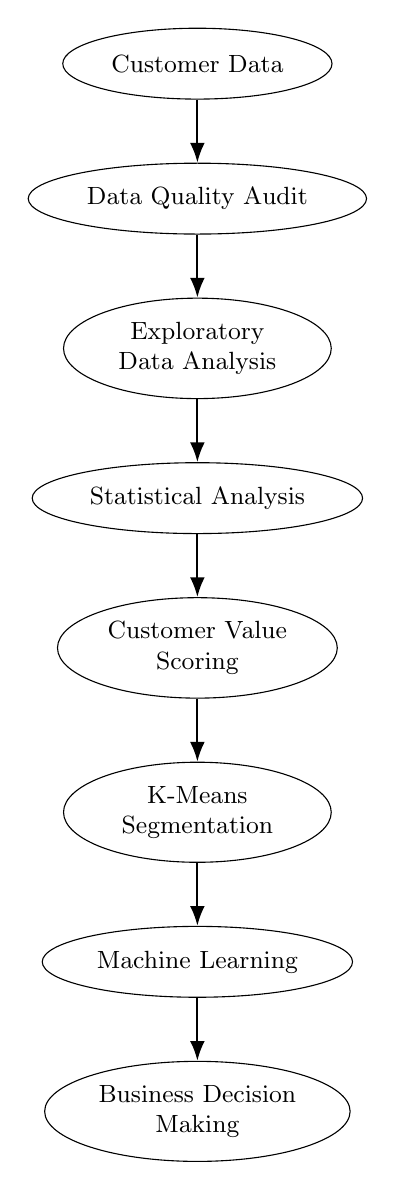
\begin{tikzpicture}[
node distance=0.8cm,
process/.style={
    draw,
    ellipse,
    minimum width=3.4cm,
    minimum height=0.9cm,
    align=center,
    font=\small
},
arrow/.style={
    -{Latex[length=2.5mm]},
    thick
}
]

\node[process] (data) {Customer Data};

\node[process, below=of data] (quality)
{Data Quality Audit};

\node[process, below=of quality] (eda)
{Exploratory\\Data Analysis};

\node[process, below=of eda] (stats)
{Statistical Analysis};

\node[process, below=of stats] (value)
{Customer Value\\Scoring};

\node[process, below=of value] (cluster)
{K-Means\\Segmentation};

\node[process, below=of cluster] (ml)
{Machine Learning};

\node[process, below=of ml] (business)
{Business Decision\\Making};

\draw[arrow] (data) -- (quality);
\draw[arrow] (quality) -- (eda);
\draw[arrow] (eda) -- (stats);
\draw[arrow] (stats) -- (value);
\draw[arrow] (value) -- (cluster);
\draw[arrow] (cluster) -- (ml);
\draw[arrow] (ml) -- (business);

\end{tikzpicture}
\caption{Integrated analytical framework used in the study}
\label{fig:workflow}
\end{figure}

The workflow combines descriptive, inferential, unsupervised, and supervised analytical techniques.

The main Python libraries used in the project include:

\begin{itemize}
    \item pandas
    \item NumPy
    \item SciPy
    \item scikit-learn
    \item matplotlib
    \item seaborn
    \item openpyxl
    \item joblib
\end{itemize}

% =========================================================
% 4 EDA
% =========================================================

\section{Exploratory Data Analysis}

Exploratory Data Analysis (EDA) was performed to characterize the distributions of customer age, purchase frequency, average order value, total spending, inactivity, and satisfaction.

Because the sample contains only 60 observations, numerical summaries were considered together with distributional diagnostics and graphical inspection.

The main numerical variables used throughout the analysis were:

\begin{itemize}
    \item Age
    \item Purchase Count
    \item Average Order Value
    \item Total Spending
    \item Last Purchase Days
    \item Satisfaction Score
\end{itemize}

The distributions indicate substantial heterogeneity, particularly in total spending and purchase behavior.

% =========================================================
% 5 NORMALITY
% =========================================================

\section{Normality and Outlier Analysis}

\subsection{Normality Testing}

The Shapiro--Wilk test was applied to assess the normality of the main numerical variables.

The null hypothesis was:

\[
\Hnull:\quad X \sim \text{Normal Distribution}.
\]

The alternative hypothesis was:

\[
\Halt:\quad X \not\sim \text{Normal Distribution}.
\]

The results are presented in Table~\ref{tab:normality}.

\begin{table}[H]
\centering
\caption{Shapiro--Wilk normality test}
\label{tab:normality}
\begin{tabular}{lcc}
\toprule
\textbf{Variable} & \textbf{W} & \textbf{p-value}\\
\midrule
Age & 0.938 & 0.004\\
Purchase Count & 0.957 & 0.033\\
Average Order Value & 0.915 & $<0.001$\\
Total Spending & 0.708 & $<0.001$\\
Last Purchase Days & 0.970 & 0.142\\
Satisfaction Score & 0.879 & $<0.001$\\
\bottomrule
\end{tabular}
\end{table}

At the 5\% significance level, most variables reject the normality hypothesis. Consequently, non-parametric statistical procedures are preferred for inferential comparisons.

\subsection{Outlier Detection}

Outliers were investigated using the Interquartile Range (IQR) criterion:

\[
IQR=Q_3-Q_1.
\]

The lower and upper bounds are defined as:

\[
L=Q_1-1.5(IQR),
\]

\[
U=Q_3+1.5(IQR).
\]

Observations outside $[L,U]$ are potential statistical outliers.

High-spending observations were not automatically removed because they may represent genuine economically important customers.

For example, Customer 1030 has:

\begin{align}
\text{Total Spending} &= 25,000,\\
\text{Purchase Count} &= 26,\\
\text{Last Purchase Days} &= 340.
\end{align}

This observation is statistically unusual but potentially highly valuable from a managerial perspective.

% =========================================================
% 6 CORRELATION
% =========================================================

\section{Correlation Analysis}

Because several variables exhibited non-normal distributions, Spearman's rank correlation coefficient was used.

Spearman's coefficient is defined as:

\[
\rho_s =
1-
\frac{6\sum d_i^2}{n(n^2-1)},
\]

where $d_i$ represents the difference between the ranks of the two variables for observation $i$.

The strongest relationships are summarized in Table~\ref{tab:correlation}.

\begin{table}[H]
\centering
\caption{Selected Spearman rank correlations}
\label{tab:correlation}
\begin{tabular}{lc}
\toprule
\textbf{Variable Pair} & \boldmath$\rho_s$\\
\midrule
Purchase Count -- Total Spending & 0.613\\
Average Order Value -- Total Spending & 0.434\\
Last Purchase Days -- Satisfaction & -0.293\\
Age -- Purchase Count & 0.265\\
\bottomrule
\end{tabular}
\end{table}

The strongest association was observed between Purchase Count and Total Spending:

\[
\rho_s=0.613.
\]

This indicates a moderate positive monotonic relationship, suggesting that customers who purchase more frequently tend to generate greater cumulative spending.

Nevertheless, correlation does not imply causation.

% =========================================================
% 7 CUSTOMER VALUE
% =========================================================

\section{Customer Value Analysis}

A composite Customer Value Score was developed using standardized versions of Total Spending, Purchase Count, and Average Order Value.

The score is defined as:

\[
CVS=
0.50Z(TS)
+
0.30Z(PC)
+
0.20Z(AOV),
\]

where:

\begin{itemize}
    \item $TS$ = Total Spending,
    \item $PC$ = Purchase Count,
    \item $AOV$ = Average Order Value.
\end{itemize}

Total Spending receives the largest weight because it represents realized customer revenue.

Customers were divided into three equal-sized value groups using empirical quantiles.

\begin{table}[H]
\centering
\caption{Customer value segments}
\label{tab:value_segments}
\begin{tabular}{lcc}
\toprule
\textbf{Segment} & \textbf{Customers} & \textbf{Share}\\
\midrule
Low Value & 20 & 33.3\%\\
Medium Value & 20 & 33.3\%\\
High Value & 20 & 33.3\%\\
\bottomrule
\end{tabular}
\end{table}

The segmentation provides a transparent basis for differentiated customer management.

% =========================================================
% 8 CHURN
% =========================================================

\section{Churn-Risk Analysis}

Churn risk was operationalized using customer inactivity.

A customer was classified as churn-risk when:

\[
\text{Last Purchase Days}>180.
\]

The resulting classification is presented in Table~\ref{tab:churn}.

\begin{table}[H]
\centering
\caption{Churn-risk classification}
\label{tab:churn}
\begin{tabular}{lcc}
\toprule
\textbf{Status} & \textbf{Customers} & \textbf{Percentage}\\
\midrule
Active & 24 & 40\%\\
Churn Risk & 36 & 60\%\\
\bottomrule
\end{tabular}
\end{table}

Thus,

\[
\frac{36}{60}\times100=60\%.
\]

A particularly important group consists of customers who are both High Value and Churn Risk.

There are 12 such customers:

\[
\frac{12}{60}\times100=20\%.
\]

This group should receive the highest retention priority.

It is important to emphasize that churn is defined here as an inactivity-based proxy rather than an observed future churn outcome.

% =========================================================
% 9 KMEANS
% =========================================================

\section{Customer Segmentation Using K-Means}

K-Means clustering was applied using:

\begin{itemize}
    \item Purchase Count,
    \item Average Order Value,
    \item Total Spending,
    \item Last Purchase Days.
\end{itemize}

The variables were standardized before clustering.

The quality of candidate cluster solutions was assessed using the silhouette coefficient.

\begin{table}[H]
\centering
\caption{Silhouette scores for candidate cluster solutions}
\label{tab:silhouette}
\begin{tabular}{cc}
\toprule
\textbf{Number of Clusters} & \textbf{Silhouette Score}\\
\midrule
2 & 0.280\\
3 & \textbf{0.316}\\
4 & 0.297\\
5 & 0.308\\
6 & 0.299\\
\bottomrule
\end{tabular}
\end{table}

The highest silhouette score occurred at $K=3$.

Therefore, three clusters were selected.

% =========================================================
% 10 CLUSTER PROFILES
% =========================================================

\section{Cluster Profiles and Statistical Validation}

The three identified clusters are summarized in Table~\ref{tab:clusters}.

\begin{table}[H]
\centering
\caption{K-Means customer cluster profiles}
\label{tab:clusters}
\begin{adjustbox}{max width=\textwidth}
\begin{tabular}{lrrrrr}
\toprule
\textbf{Cluster} &
\textbf{Customers} &
\textbf{Avg. Purchases} &
\textbf{Avg. AOV} &
\textbf{Avg. Spending} &
\textbf{Avg. Inactivity}\\
\midrule
Cluster 0 & 6 & 30.33 & 348.60 & 14,188.76 & 211.17\\
Cluster 1 & 23 & 8.30 & 309.07 & 2,603.76 & 232.17\\
Cluster 2 & 31 & 21.61 & 115.78 & 2,475.26 & 173.81\\
\bottomrule
\end{tabular}
\end{adjustbox}
\end{table}

\subsection{Cluster 0: Premium Customers}

Cluster 0 contains only six customers but has an average total spending of approximately 14,188.76.

This cluster represents the company's most economically valuable behavioral group.

Recommended strategies include VIP retention, personalized communication, premium services, early access, and targeted relationship management.

\subsection{Cluster 1: Low-Frequency Customers}

Cluster 1 contains 23 customers with an average purchase count of 8.30 and average inactivity of approximately 232 days.

This group is suitable for reactivation strategies and personalized engagement.

\subsection{Cluster 2: Frequent Low-Basket Customers}

Cluster 2 contains 31 customers with relatively high purchase frequency but an average order value of only 115.78.

This segment provides a strong opportunity for cross-selling, bundling, and upselling.

\subsection{Kruskal--Wallis Validation}

To statistically evaluate whether total spending differs across clusters, the Kruskal--Wallis test was applied.

The test statistic was:

\[
H=16.109,
\]

with:

\[
p=0.000318.
\]

Since:

\[
p<0.05,
\]

the null hypothesis of identical spending distributions across the clusters is rejected.

Therefore, statistically significant differences in customer spending exist across the identified segments.

% =========================================================
% 11 MACHINE LEARNING
% =========================================================

\section{Machine-Learning Churn Analysis}

Two supervised learning algorithms were evaluated:

\begin{enumerate}
    \item Logistic Regression
    \item Random Forest
\end{enumerate}

Predictors included:

\begin{itemize}
    \item Age
    \item Purchase Count
    \item Average Order Value
    \item Total Spending
    \item Satisfaction Score
    \item Returned Items
\end{itemize}

The variable \texttt{last\_purchase\_days} was excluded because it directly defines the churn target. Including it would introduce target leakage.

\subsection{Cross-Validation Results}

Stratified five-fold cross-validation was used.

\begin{table}[H]
\centering
\caption{Cross-validated machine-learning performance}
\label{tab:ml}
\begin{tabular}{lcc}
\toprule
\textbf{Model} & \textbf{Mean ROC-AUC} & \textbf{Std. Dev.}\\
\midrule
Logistic Regression & \textbf{0.564} & 0.084\\
Random Forest & 0.478 & 0.096\\
\bottomrule
\end{tabular}
\end{table}

The results indicate weak predictive performance.

A ROC-AUC value near 0.50 corresponds approximately to random classification. Logistic Regression performs somewhat better than Random Forest, but neither model is sufficiently strong for production deployment.

% =========================================================
% 12 FEATURE IMPORTANCE
% =========================================================

\section{Random Forest Feature Importance}

The estimated Random Forest feature importances are presented in Table~\ref{tab:importance}.

\begin{table}[H]
\centering
\caption{Random Forest feature importance}
\label{tab:importance}
\begin{tabular}{lr}
\toprule
\textbf{Feature} & \textbf{Importance}\\
\midrule
Total Spending & 0.235\\
Average Order Value & 0.214\\
Satisfaction Score & 0.167\\
Age & 0.156\\
Purchase Count & 0.149\\
Returned Items & 0.078\\
\bottomrule
\end{tabular}
\end{table}

Total Spending and Average Order Value were the two most influential variables within the fitted Random Forest.

These importance values should not be interpreted as causal effects.

% =========================================================
% 13 DISCOUNT
% =========================================================

\section{Discount Effectiveness Analysis}

Customers were divided into discount users and non-users.

\begin{table}[H]
\centering
\caption{Descriptive comparison of discount groups}
\label{tab:discount}
\begin{tabular}{lcc}
\toprule
\textbf{Metric} & \textbf{Discount} & \textbf{No Discount}\\
\midrule
Customers & 26 & 34\\
Mean Total Spending & 3,642.42 & 3,736.74\\
Mean AOV & 203.29 & 220.70\\
Mean Satisfaction & 3.27 & 2.76\\
\bottomrule
\end{tabular}
\end{table}

Because the data are non-normal, the Mann--Whitney U test was applied.

The results were:

\[
U=391,
\]

\[
p=0.4512.
\]

Since:

\[
p>0.05,
\]

there is no statistically significant evidence of a difference in total spending between the two groups.

The estimated Cohen's $d$ was approximately:

\[
d=-0.022.
\]

The bootstrap 95\% confidence interval for the mean spending difference was approximately:

\[
[-2146.19,\;2400.88].
\]

Because the confidence interval contains zero, the data do not provide strong evidence of a systematic spending difference.

Importantly, this does not demonstrate that discounts are ineffective. The observational design does not establish causality.

% =========================================================
% 14 CITY
% =========================================================

\section{City-Level Marketing Opportunity}

City-level marketing opportunity was evaluated using customer count, total revenue, average customer value, and satisfaction.

Table~\ref{tab:city} presents the principal city-level results.

\begin{table}[H]
\centering
\caption{Selected city-level customer and revenue indicators}
\label{tab:city}
\begin{adjustbox}{max width=\textwidth}
\begin{tabular}{lrrrr}
\toprule
\textbf{City} &
\textbf{Customers} &
\textbf{Total Revenue} &
\textbf{Avg. Spending} &
\textbf{Avg. Satisfaction}\\
\midrule
Mashhad & 11 & 64,118.44 & 5,828.95 & 2.91\\
Tabriz & 12 & 36,192.49 & 3,016.04 & 3.00\\
Karaj & 7 & 26,189.81 & 3,741.40 & 2.86\\
Ahvaz & 8 & 23,384.78 & 2,923.10 & 3.50\\
Isfahan & 5 & 21,975.32 & 4,395.06 & 4.40\\
Shiraz & 6 & 20,715.92 & 3,452.65 & 2.00\\
Rasht & 5 & 15,168.54 & 3,033.71 & 2.60\\
Tehran & 6 & 14,006.85 & 2,334.48 & 2.67\\
\bottomrule
\end{tabular}
\end{adjustbox}
\end{table}

Mashhad achieved the highest observed total revenue:

\[
R_{\text{Mashhad}}=64,118.44.
\]

It also recorded the highest average customer spending among the listed cities.

Therefore, Mashhad represents the strongest candidate for a controlled marketing experiment.

However, the average satisfaction score of 2.91 indicates that customer-experience problems should be investigated before aggressively scaling acquisition.

% =========================================================
% 15 BUSINESS RECOMMENDATIONS
% =========================================================

\section{Business Recommendations}

The analytical results lead to three principal recommendations.

\subsection{Recommendation 1: High-Value Customer Retention}

The company should immediately prioritize the 12 customers who are both High Value and Churn Risk.

Potential actions include:

\begin{itemize}
    \item Personalized communication
    \item VIP benefits
    \item Exclusive product recommendations
    \item Early product access
    \item Personalized incentives
    \item Customer-service follow-up
\end{itemize}

The main performance indicators should include:

\begin{itemize}
    \item Reactivation Rate
    \item Revenue Recovered
    \item Repeat Purchase Rate
    \item Customer Lifetime Value
    \item Cost per Reactivated Customer
\end{itemize}

\subsection{Recommendation 2: Increase Average Order Value}

The 31 customers in Cluster 2 represent a major upselling opportunity.

Recommended tactics include:

\begin{itemize}
    \item Product bundles
    \item Cross-selling
    \item Complementary-product recommendations
    \item Free-shipping thresholds
    \item Quantity-based offers
    \item Premium-product recommendations
\end{itemize}

The primary KPI should be Average Order Value.

\subsection{Recommendation 3: Controlled Marketing Experiment in Mashhad}

Mashhad should be considered for a controlled marketing pilot.

A randomized experimental design is recommended:

\begin{center}
\begin{tikzpicture}[
node distance=1.2cm,
process/.style={
    draw,
    ellipse,
    minimum width=3.5cm,
    minimum height=0.9cm,
    align=center
},
arrow/.style={-{Latex[length=2.5mm]}, thick}
]

\node[process] (customers) {Eligible Customers};
\node[process, below left=of customers] (control) {Control Group};
\node[process, below right=of customers] (treat) {Campaign Group};
\node[process, below=1.5cm of control] (cresult) {Revenue / Conversion};
\node[process, below=1.5cm of treat] (tresult) {Revenue / Conversion};
\node[process, below=1.5cm of $(cresult)!0.5!(tresult)$] (decision) {Incremental ROI};

\draw[arrow] (customers) -- (control);
\draw[arrow] (customers) -- (treat);
\draw[arrow] (control) -- (cresult);
\draw[arrow] (treat) -- (tresult);
\draw[arrow] (cresult) -- (decision);
\draw[arrow] (tresult) -- (decision);

\end{tikzpicture}
\end{center}

The experiment should evaluate incremental revenue, conversion, repeat purchasing, customer satisfaction, and Return on Advertising Spend (ROAS).

% =========================================================
% 16 STRATEGY MATRIX
% =========================================================

\section{Customer Strategy Matrix}

\begin{table}[H]
\centering
\caption{Recommended customer-management strategies}
\label{tab:strategy}
\begin{adjustbox}{max width=\textwidth}
\begin{tabular}{p{3.3cm}p{4cm}p{5cm}}
\toprule
\textbf{Customer Type} &
\textbf{Main Problem} &
\textbf{Recommended Action}\\
\midrule
High Value + Churn Risk &
Risk of losing high revenue &
Immediate personalized retention\\

High Value + Active &
Protect existing value &
VIP loyalty and relationship management\\

Frequent + Low AOV &
Low basket size &
Upselling and cross-selling\\

Low Frequency + Churn Risk &
Low engagement &
Reactivation campaign\\

Discount Users &
Unclear incremental value &
Targeted A/B-tested discounts\\

Mashhad Customers &
High commercial opportunity &
Controlled marketing experiment\\
\bottomrule
\end{tabular}
\end{adjustbox}
\end{table}

% =========================================================
% 17 LIMITATIONS
% =========================================================

\section{Limitations}

\subsection{Small Sample Size}

The dataset contains only 60 customers. Consequently, machine-learning estimates may be unstable and should be considered exploratory.

\subsection{Proxy Churn Definition}

Churn was defined using:

\[
\text{Last Purchase Days}>180.
\]

This is a business-rule proxy rather than an observed future churn event.

\subsection{Observational Discount Analysis}

Customers were not randomly assigned to discount and non-discount groups. Therefore, causal conclusions about discount effectiveness cannot be established.

\subsection{Potential Sampling Bias}

The available customer sample may not represent the complete customer population.

\subsection{Machine-Learning Performance}

The Logistic Regression model achieved a mean ROC-AUC of approximately 0.564, while Random Forest achieved approximately 0.478.

These results do not justify production deployment.

% =========================================================
% 18 FUTURE RESEARCH
% =========================================================

\section{Future Research}

A production-level customer analytics system should incorporate longitudinal transaction data.

Important additional variables include:

\begin{itemize}
    \item Transaction timestamps
    \item Product identifiers
    \item Product categories
    \item Quantity
    \item Price
    \item Discount amount
    \item Gross revenue
    \item Profit margin
    \item Website sessions
    \item App activity
    \item Cart abandonment
    \item Email engagement
    \item Campaign exposure
\end{itemize}

A genuine churn target should be defined as a future behavioral outcome.

For example:

\[
Y_i=
\begin{cases}
1, & \text{if customer }i\text{ does not purchase during the future window},\\
0, & \text{otherwise}.
\end{cases}
\]

A temporal train-test split should then be used to estimate true out-of-time predictive performance.

Potential future algorithms include:

\begin{itemize}
    \item Logistic Regression
    \item Random Forest
    \item Gradient Boosting
    \item XGBoost
    \item Survival Analysis
\end{itemize}

Performance should be evaluated using ROC-AUC, Precision-Recall AUC (PR-AUC), calibration, and business-cost metrics.

% =========================================================
% 19 CONCLUSION
% =========================================================

\section{Conclusion}

This study demonstrates how customer-level data can be transformed into actionable business intelligence through an integrated statistical and machine-learning framework.

The analysis revealed substantial heterogeneity in customer value. Twenty customers were classified as High Value, while K-Means clustering identified a particularly valuable behavioral segment containing only six customers with an average total spending of approximately 14,188.76.

The churn-risk analysis identified 36 inactive customers, representing 60\% of the sample under the selected inactivity rule. More importantly, 12 customers were simultaneously classified as High Value and Churn Risk. These customers represent the most strategically important retention group.

The K-Means segmentation was supported by the Kruskal--Wallis test, which produced:

\[
H=16.109,\qquad p=0.000318.
\]

Thus, customer spending differs significantly across the identified behavioral segments.

The discount analysis did not detect a statistically significant spending difference:

\[
U=391,\qquad p=0.4512.
\]

Consequently, broad discounting cannot be justified based solely on the current observational evidence. Controlled experiments are recommended to estimate the incremental effect of discounts.

At the geographical level, Mashhad achieved the highest observed total revenue of approximately 64,118.44. However, its moderate satisfaction level indicates that marketing expansion should be accompanied by improvements in customer experience.

The machine-learning results were limited. Logistic Regression achieved a mean cross-validated ROC-AUC of approximately 0.564, whereas Random Forest achieved 0.478. These findings indicate that the current dataset is not sufficiently large or longitudinal for reliable production churn prediction.

Overall, the evidence supports a differentiated customer strategy rather than a one-size-fits-all marketing approach.

The recommended priority is therefore:

\[
\boxed{
\text{Protect High-Value Customers}
\rightarrow
\text{Increase AOV}
\rightarrow
\text{Validate Marketing Through Experiments}
}
\]

This framework provides a practical foundation for future customer analytics systems once larger and longitudinal datasets become available.

% =========================================================
% 20 MANAGEMENT ACTION PLAN
% =========================================================

\section{Final Management Action Plan}

\begin{table}[H]
\centering
\caption{Prioritized management action plan}
\label{tab:action_plan}
\begin{adjustbox}{max width=\textwidth}
\begin{tabular}{clll}
\toprule
\textbf{Priority} &
\textbf{Action} &
\textbf{Target} &
\textbf{Primary KPI}\\
\midrule
1 &
High-value retention &
12 High Value + Churn Risk &
Reactivation Rate\\

2 &
Upselling and cross-selling &
31 frequent low-AOV customers &
Average Order Value\\

3 &
Marketing pilot &
Mashhad &
Incremental Revenue / ROI\\

4 &
Discount A/B testing &
Selected customer groups &
Revenue Lift\\

5 &
Improve churn data &
All customers &
Future ROC-AUC / PR-AUC\\
\bottomrule
\end{tabular}
\end{adjustbox}
\end{table}

The principal managerial conclusion is that customer resources should be allocated according to economic value, behavioral characteristics, and risk rather than treating all customers identically.

% =========================================================
% REFERENCES
% =========================================================

\begin{thebibliography}{99}

\bibitem{scikit}
Pedregosa, F., Varoquaux, G., Gramfort, A., et al.
Scikit-learn: Machine Learning in Python.
\textit{Journal of Machine Learning Research}, 12, 2825--2830, 2011.

\bibitem{spearman}
Spearman, C.
The proof and measurement of association between two things.
\textit{The American Journal of Psychology}, 15(1), 72--101, 1904.

\bibitem{kmeans}
MacQueen, J.
Some methods for classification and analysis of multivariate observations.
In \textit{Proceedings of the Fifth Berkeley Symposium on Mathematical Statistics and Probability}, 1967.

\bibitem{silhouette}
Rousseeuw, P. J.
Silhouettes: A graphical aid to the interpretation and validation of cluster analysis.
\textit{Journal of Computational and Applied Mathematics}, 20, 53--65, 1987.

\bibitem{mannwhitney}
Mann, H. B., \& Whitney, D. R.
On a test of whether one of two random variables is stochastically larger than the other.
\textit{The Annals of Mathematical Statistics}, 18(1), 50--60, 1947.

\bibitem{shapiro}
Shapiro, S. S., \& Wilk, M. B.
An analysis of variance test for normality.
\textit{Biometrika}, 52(3--4), 591--611, 1965.

\end{thebibliography}

\end{document}
